\documentclass[11pt]{article}

% Call the style package
%\usepackage{fun3style}

\title{Quaternion Neural Networks for 3D Sound Source Localization in Reverberant Environments: Implementation with First Order Ambisonics}
\author{Roberto Aureli, ID 1757131\\
		Riccardo Caprari, ID 1743168\\
		Gianmarco Fioretti, ID 1762135}

\date{Neural Networks, Winter 2020}



\usepackage{graphicx}

\graphicspath{{./img/}}

\usepackage[utf8]{inputenc}
\usepackage[english]{babel}


\usepackage{xcolor}
\usepackage{nth}
\usepackage{amsmath}
\usepackage{relsize}
\usepackage{wrapfig}
\usepackage{float}
\usepackage{hyperref}
\usepackage{listings}


\usepackage{caption}



\usepackage{wrapfig}
\usepackage{csquotes}
\usepackage{float}
\usepackage{amssymb}
\usepackage{multicol}
\usepackage{ragged2e}



\usepackage{indentfirst}

\setlength{\parindent}{2em}
\setlength{\parskip}{1em}




\begin{document}



\maketitle

\vspace{10px}

\openup -1.5ex
\tableofcontents
\openup 1.5ex

\newpage
\section{Introduction}\label{cha:intro}

This project addresses the \textbf{3D Sound Event Localization and Detection Task} in reverberant environments with a  quaternion neural network (deep neural network with quaternion input features extracted from the acoustic intensity vector).\newline

As mentioned above, the proposed model performs both sound localization and sound event detection and subsequent classification. In particular it follows the architecture described in 2020 paper (TO ADD REFERENCE) which allows to estimate the three-dimensional direction of arrivals (DOA), in addition, it has been modified in order to be capable of detecting sound events and estimating the corresponding sources (eleven different classes provided by the development dataset, check for Table \ref{table:classes}).\newline

Many recent works have proven that deep quaternion neural networks are able to improve localization performances dramatically, especially in reverberant and noisy environments, thanks to spatial harmonic decomposition which permits to exploit the intrinsic correlation of the ambisonics signal components. One of the main aspect to be considered is the input features to be passed to the network (TO FILL).\newline

Our main work consisted in adapting the provided code to the new dataset, fine-tuning the model's hyper-parameters, applying the three metrics defined in the 2019 paper  (TO ADD REFERENCE) (\textbf{SED, DOA, SELD}), implementing the direction of arrival estimation in spherical coordinates, and computing the confidence intervals on the model's final errors as defined in the 2018 paper (TO ADD REFERENCE) in order to add also a statistical evaluation on final results.


\section{Dataset}\label{cha:data}

The network is trained with the \textbf{TAU Spatial Sound Events 2019} dataset which provides four-channel directional microphone recordings of stationary point sources.\\
It is a balanced dataset, it indeed consists of eleven classes, each with twenty examples that were randomly split into five sets with an equal number of examples for each class, in addition, it was divided into four cross-validation split.\\
The maximum number of simultaneously overlapping sources are two.\\
Moreover, in order to improve the performance over new sound events, and to make a more realistic scenario, natural ambient noise collected in the recording locations was added to the synthesized recordings in the dataset such that the average SNR of the sound events was 30 dB.

\begin{table}[ht]
	\caption{TAU Spatial Sound Events Classes}
	\centering
	\begin{tabular}{c c}
		\hline\hline
		Sound class & Index \\ [0.5ex]
		\hline
		knock & 0 \\
		drawer & 1 \\
		clearthroat & 2 \\
		phone & 3 \\
		keysDrop & 4 \\
		speech & 5 \\
		keyboard & 6 \\
		pageturn & 7 \\
		cough & 8 \\
		doorslam & 9 \\
		laughter & 10\\
		\hline		
	\end{tabular}
	\label{table:classes}
\end{table}


\section{Architecture}\label{cha:arch}

The network proposed in the 2020 paper (TO ADD REFERENCE) involves a series of convolutional layers in the quaternion domains, they are composed of several filter kernels which allow learning inter-channel features, with subsequent activation functions (TO FILL) and max-pooling functions. The output of this series are properly reshaped and fed to bidirectional quaternion recurrent layers. This first part of the architecture is depicted in Figure \ref{fig:arch1}

\begin{figure}[ht]
	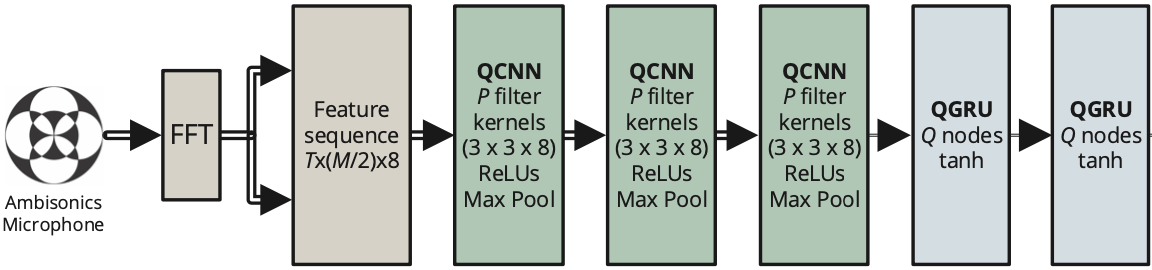
\includegraphics[width=\linewidth]{img/arch1.png}
	\caption{First part of the Network Architecture}
	\label{fig:arch1}
\end{figure}

As already pointed out on Chapter \ref{cha:intro} the network has been modified accordingly, the final part of architecture therefore becomes as in Figure \ref{fig:arch2}, so that network is able to perform a multi-classification for the SED task (one for each class: 1 to indicate detection, 0 otherwise) and multi-regressions for DOA task (one for the azimuth angle, one for the elevation angle and one for the distance.

\begin{figure}[ht]
	\centering
	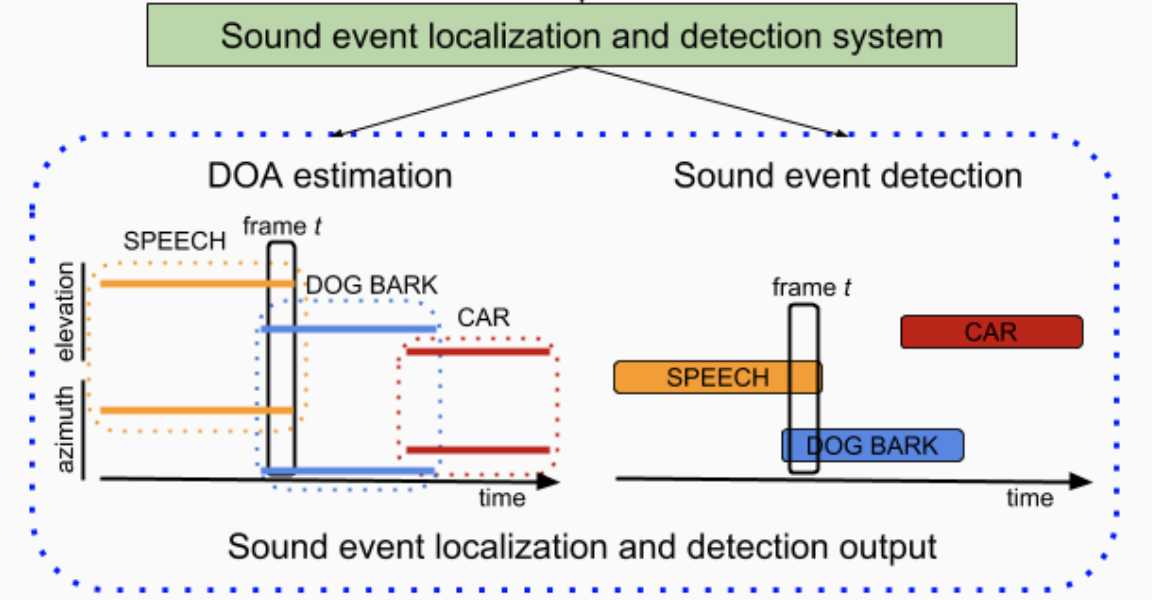
\includegraphics[scale=0.5]{img/arch2.png}
	\caption{Last part of the Network Architecture}
	\label{fig:arch2}
\end{figure}


\section{OUR WORK}

TO ADD OUR WORK


\section{Results}\label{cha:res}

TO ADD RESULTS

\section{Conclusions}\label{cha:conc}

TO ADD CONCLUSIONS

\newpage

TO ADD REFERENCES

\end{document}
